% Options for packages loaded elsewhere
% Options for packages loaded elsewhere
\PassOptionsToPackage{unicode}{hyperref}
\PassOptionsToPackage{hyphens}{url}
\PassOptionsToPackage{dvipsnames,svgnames,x11names}{xcolor}
%
\documentclass[
  letterpaper,
  DIV=11,
  numbers=noendperiod]{scrartcl}
\usepackage{xcolor}
\usepackage{amsmath,amssymb}
\setcounter{secnumdepth}{-\maxdimen} % remove section numbering
\usepackage{iftex}
\ifPDFTeX
  \usepackage[T1]{fontenc}
  \usepackage[utf8]{inputenc}
  \usepackage{textcomp} % provide euro and other symbols
\else % if luatex or xetex
  \usepackage{unicode-math} % this also loads fontspec
  \defaultfontfeatures{Scale=MatchLowercase}
  \defaultfontfeatures[\rmfamily]{Ligatures=TeX,Scale=1}
\fi
\usepackage{lmodern}
\ifPDFTeX\else
  % xetex/luatex font selection
\fi
% Use upquote if available, for straight quotes in verbatim environments
\IfFileExists{upquote.sty}{\usepackage{upquote}}{}
\IfFileExists{microtype.sty}{% use microtype if available
  \usepackage[]{microtype}
  \UseMicrotypeSet[protrusion]{basicmath} % disable protrusion for tt fonts
}{}
\makeatletter
\@ifundefined{KOMAClassName}{% if non-KOMA class
  \IfFileExists{parskip.sty}{%
    \usepackage{parskip}
  }{% else
    \setlength{\parindent}{0pt}
    \setlength{\parskip}{6pt plus 2pt minus 1pt}}
}{% if KOMA class
  \KOMAoptions{parskip=half}}
\makeatother
% Make \paragraph and \subparagraph free-standing
\makeatletter
\ifx\paragraph\undefined\else
  \let\oldparagraph\paragraph
  \renewcommand{\paragraph}{
    \@ifstar
      \xxxParagraphStar
      \xxxParagraphNoStar
  }
  \newcommand{\xxxParagraphStar}[1]{\oldparagraph*{#1}\mbox{}}
  \newcommand{\xxxParagraphNoStar}[1]{\oldparagraph{#1}\mbox{}}
\fi
\ifx\subparagraph\undefined\else
  \let\oldsubparagraph\subparagraph
  \renewcommand{\subparagraph}{
    \@ifstar
      \xxxSubParagraphStar
      \xxxSubParagraphNoStar
  }
  \newcommand{\xxxSubParagraphStar}[1]{\oldsubparagraph*{#1}\mbox{}}
  \newcommand{\xxxSubParagraphNoStar}[1]{\oldsubparagraph{#1}\mbox{}}
\fi
\makeatother

\usepackage{color}
\usepackage{fancyvrb}
\newcommand{\VerbBar}{|}
\newcommand{\VERB}{\Verb[commandchars=\\\{\}]}
\DefineVerbatimEnvironment{Highlighting}{Verbatim}{commandchars=\\\{\}}
% Add ',fontsize=\small' for more characters per line
\usepackage{framed}
\definecolor{shadecolor}{RGB}{241,243,245}
\newenvironment{Shaded}{\begin{snugshade}}{\end{snugshade}}
\newcommand{\AlertTok}[1]{\textcolor[rgb]{0.68,0.00,0.00}{#1}}
\newcommand{\AnnotationTok}[1]{\textcolor[rgb]{0.37,0.37,0.37}{#1}}
\newcommand{\AttributeTok}[1]{\textcolor[rgb]{0.40,0.45,0.13}{#1}}
\newcommand{\BaseNTok}[1]{\textcolor[rgb]{0.68,0.00,0.00}{#1}}
\newcommand{\BuiltInTok}[1]{\textcolor[rgb]{0.00,0.23,0.31}{#1}}
\newcommand{\CharTok}[1]{\textcolor[rgb]{0.13,0.47,0.30}{#1}}
\newcommand{\CommentTok}[1]{\textcolor[rgb]{0.37,0.37,0.37}{#1}}
\newcommand{\CommentVarTok}[1]{\textcolor[rgb]{0.37,0.37,0.37}{\textit{#1}}}
\newcommand{\ConstantTok}[1]{\textcolor[rgb]{0.56,0.35,0.01}{#1}}
\newcommand{\ControlFlowTok}[1]{\textcolor[rgb]{0.00,0.23,0.31}{\textbf{#1}}}
\newcommand{\DataTypeTok}[1]{\textcolor[rgb]{0.68,0.00,0.00}{#1}}
\newcommand{\DecValTok}[1]{\textcolor[rgb]{0.68,0.00,0.00}{#1}}
\newcommand{\DocumentationTok}[1]{\textcolor[rgb]{0.37,0.37,0.37}{\textit{#1}}}
\newcommand{\ErrorTok}[1]{\textcolor[rgb]{0.68,0.00,0.00}{#1}}
\newcommand{\ExtensionTok}[1]{\textcolor[rgb]{0.00,0.23,0.31}{#1}}
\newcommand{\FloatTok}[1]{\textcolor[rgb]{0.68,0.00,0.00}{#1}}
\newcommand{\FunctionTok}[1]{\textcolor[rgb]{0.28,0.35,0.67}{#1}}
\newcommand{\ImportTok}[1]{\textcolor[rgb]{0.00,0.46,0.62}{#1}}
\newcommand{\InformationTok}[1]{\textcolor[rgb]{0.37,0.37,0.37}{#1}}
\newcommand{\KeywordTok}[1]{\textcolor[rgb]{0.00,0.23,0.31}{\textbf{#1}}}
\newcommand{\NormalTok}[1]{\textcolor[rgb]{0.00,0.23,0.31}{#1}}
\newcommand{\OperatorTok}[1]{\textcolor[rgb]{0.37,0.37,0.37}{#1}}
\newcommand{\OtherTok}[1]{\textcolor[rgb]{0.00,0.23,0.31}{#1}}
\newcommand{\PreprocessorTok}[1]{\textcolor[rgb]{0.68,0.00,0.00}{#1}}
\newcommand{\RegionMarkerTok}[1]{\textcolor[rgb]{0.00,0.23,0.31}{#1}}
\newcommand{\SpecialCharTok}[1]{\textcolor[rgb]{0.37,0.37,0.37}{#1}}
\newcommand{\SpecialStringTok}[1]{\textcolor[rgb]{0.13,0.47,0.30}{#1}}
\newcommand{\StringTok}[1]{\textcolor[rgb]{0.13,0.47,0.30}{#1}}
\newcommand{\VariableTok}[1]{\textcolor[rgb]{0.07,0.07,0.07}{#1}}
\newcommand{\VerbatimStringTok}[1]{\textcolor[rgb]{0.13,0.47,0.30}{#1}}
\newcommand{\WarningTok}[1]{\textcolor[rgb]{0.37,0.37,0.37}{\textit{#1}}}

\usepackage{longtable,booktabs,array}
\usepackage{calc} % for calculating minipage widths
% Correct order of tables after \paragraph or \subparagraph
\usepackage{etoolbox}
\makeatletter
\patchcmd\longtable{\par}{\if@noskipsec\mbox{}\fi\par}{}{}
\makeatother
% Allow footnotes in longtable head/foot
\IfFileExists{footnotehyper.sty}{\usepackage{footnotehyper}}{\usepackage{footnote}}
\makesavenoteenv{longtable}
\usepackage{graphicx}
\makeatletter
\newsavebox\pandoc@box
\newcommand*\pandocbounded[1]{% scales image to fit in text height/width
  \sbox\pandoc@box{#1}%
  \Gscale@div\@tempa{\textheight}{\dimexpr\ht\pandoc@box+\dp\pandoc@box\relax}%
  \Gscale@div\@tempb{\linewidth}{\wd\pandoc@box}%
  \ifdim\@tempb\p@<\@tempa\p@\let\@tempa\@tempb\fi% select the smaller of both
  \ifdim\@tempa\p@<\p@\scalebox{\@tempa}{\usebox\pandoc@box}%
  \else\usebox{\pandoc@box}%
  \fi%
}
% Set default figure placement to htbp
\def\fps@figure{htbp}
\makeatother





\setlength{\emergencystretch}{3em} % prevent overfull lines

\providecommand{\tightlist}{%
  \setlength{\itemsep}{0pt}\setlength{\parskip}{0pt}}



 


\KOMAoption{captions}{tableheading}
\makeatletter
\@ifpackageloaded{tcolorbox}{}{\usepackage[skins,breakable]{tcolorbox}}
\@ifpackageloaded{fontawesome5}{}{\usepackage{fontawesome5}}
\definecolor{quarto-callout-color}{HTML}{909090}
\definecolor{quarto-callout-note-color}{HTML}{0758E5}
\definecolor{quarto-callout-important-color}{HTML}{CC1914}
\definecolor{quarto-callout-warning-color}{HTML}{EB9113}
\definecolor{quarto-callout-tip-color}{HTML}{00A047}
\definecolor{quarto-callout-caution-color}{HTML}{FC5300}
\definecolor{quarto-callout-color-frame}{HTML}{acacac}
\definecolor{quarto-callout-note-color-frame}{HTML}{4582ec}
\definecolor{quarto-callout-important-color-frame}{HTML}{d9534f}
\definecolor{quarto-callout-warning-color-frame}{HTML}{f0ad4e}
\definecolor{quarto-callout-tip-color-frame}{HTML}{02b875}
\definecolor{quarto-callout-caution-color-frame}{HTML}{fd7e14}
\makeatother
\makeatletter
\@ifpackageloaded{caption}{}{\usepackage{caption}}
\AtBeginDocument{%
\ifdefined\contentsname
  \renewcommand*\contentsname{Table of contents}
\else
  \newcommand\contentsname{Table of contents}
\fi
\ifdefined\listfigurename
  \renewcommand*\listfigurename{List of Figures}
\else
  \newcommand\listfigurename{List of Figures}
\fi
\ifdefined\listtablename
  \renewcommand*\listtablename{List of Tables}
\else
  \newcommand\listtablename{List of Tables}
\fi
\ifdefined\figurename
  \renewcommand*\figurename{Figure}
\else
  \newcommand\figurename{Figure}
\fi
\ifdefined\tablename
  \renewcommand*\tablename{Table}
\else
  \newcommand\tablename{Table}
\fi
}
\@ifpackageloaded{float}{}{\usepackage{float}}
\floatstyle{ruled}
\@ifundefined{c@chapter}{\newfloat{codelisting}{h}{lop}}{\newfloat{codelisting}{h}{lop}[chapter]}
\floatname{codelisting}{Listing}
\newcommand*\listoflistings{\listof{codelisting}{List of Listings}}
\makeatother
\makeatletter
\makeatother
\makeatletter
\@ifpackageloaded{caption}{}{\usepackage{caption}}
\@ifpackageloaded{subcaption}{}{\usepackage{subcaption}}
\makeatother
\usepackage{bookmark}
\IfFileExists{xurl.sty}{\usepackage{xurl}}{} % add URL line breaks if available
\urlstyle{same}
\hypersetup{
  pdftitle={Lab 1 Instructions},
  pdfauthor={Nicky Wakim},
  colorlinks=true,
  linkcolor={blue},
  filecolor={Maroon},
  citecolor={Blue},
  urlcolor={Blue},
  pdfcreator={LaTeX via pandoc}}


\title{Lab 1 Instructions}
\usepackage{etoolbox}
\makeatletter
\providecommand{\subtitle}[1]{% add subtitle to \maketitle
  \apptocmd{\@title}{\par {\large #1 \par}}{}{}
}
\makeatother
\subtitle{BSTA 513/613}
\author{Nicky Wakim}
\date{}
\begin{document}
\maketitle


This project includes analysis on food insecurity. Please let Nicky know
if this is a triggering topic for you. I can find a different dataset
for you to work on!

\begin{tcolorbox}[enhanced jigsaw, toptitle=1mm, toprule=.15mm, leftrule=.75mm, bottomtitle=1mm, breakable, opacityback=0, titlerule=0mm, title=\textcolor{quarto-callout-caution-color}{\faFire}\hspace{0.5em}{Caution}, arc=.35mm, colback=white, rightrule=.15mm, left=2mm, colbacktitle=quarto-callout-caution-color!10!white, coltitle=black, opacitybacktitle=0.6, colframe=quarto-callout-caution-color-frame, bottomrule=.15mm]

This lab is NOT ready to be worked on!! (3/30/2026)

\end{tcolorbox}

\subsection{Directions}\label{directions}

\href{https://github.com/nwakim/BSTA_513_S25/blob/main/project/LastName_FirstInit_Lab_01.qmd}{You
can download the \texttt{.qmd} file for this lab here.}

The above link will take you to your \textbf{editing} file.
\textbf{Please do not remove anything from this editing file!!} You will
only add your code and work to this file.

\subsection{Lab activities}\label{lab-activities}

\begin{tcolorbox}[enhanced jigsaw, toptitle=1mm, toprule=.15mm, leftrule=.75mm, bottomtitle=1mm, breakable, opacityback=0, titlerule=0mm, title=\textcolor{quarto-callout-note-color}{\faInfo}\hspace{0.5em}{Note}, arc=.35mm, colback=white, rightrule=.15mm, left=2mm, colbacktitle=quarto-callout-note-color!10!white, coltitle=black, opacitybacktitle=0.6, colframe=quarto-callout-note-color-frame, bottomrule=.15mm]

I have left it up to you to load the needed packages for this lab.

\end{tcolorbox}

\subsubsection{Reading and listening
activities}\label{reading-and-listening-activities}

I will not check that you have read or listened to any of these, but it
is a good starting point for understanding the context of our data: food
insecurity in the United States. I haven't fully read them all yet, but
I will be reading and sharing throughout the quarter.

Here are some articles:

\begin{itemize}
\item
  NPR:
  \href{https://www.npr.org/sections/health-shots/2023/10/26/1208760054/food-insecurity-families-struggle-hunger-poverty}{Millions
  of American families struggle to get food on the table, report finds}

  \begin{itemize}
  \tightlist
  \item
    With option to listen to article
  \end{itemize}
\item
  \href{https://bmcpublichealth.biomedcentral.com/articles/10.1186/s12889-021-11465-6\#Tab2}{Identification
  of factors related to food insecurity and the implications for social
  determinants of health screenings}
\item
  \href{https://www.nhlbi.nih.gov/events/2021/food-insecurity-neighborhood-food-environment-and-nutrition-health-disparities}{NIH's
  page: Food Insecurity, Neighborhood Food Environment, and Nutrition
  Health Disparities: State of the Science}
\item
  \href{https://www.ncbi.nlm.nih.gov/pmc/articles/PMC5422031/}{Food
  Insecurity among American Indians and Alaska Natives: A National
  Profile using the Current Population Survey--Food Security Supplement}
\item
  \href{https://journals.sagepub.com/doi/10.1177/21501327211052204}{A
  Framework for Evaluating Social Determinants of Health Screening and
  Referrals for Assistance}
\end{itemize}

\subsubsection{Familiarize yourself with the Well-Being and Basic Needs
Survey}\label{familiarize-yourself-with-the-well-being-and-basic-needs-survey}

Please read the
\href{https://www.urban.org/policy-centers/health-policy-center/projects/well-being-and-basic-needs-survey}{Urban
Institute's page} on the Well-Being and Basic Needs Survey (WBNS) and
more of their
\href{https://www.urban.org/sites/default/files/publication/98919/the_well-being_and_basic_needs_survey_1.pdf}{published
information of the survey} (at least the first 4 pages). You can also
read about the overarching
\href{https://www.urban.org/tags/safety-net-solid-ground\#about}{From
Safety Net to Solid Ground Initiative} that started the survey. Answer
the following questions:

\begin{itemize}
\tightlist
\item
  What is the motivation for this study?
\item
  How could an analysis that looks at associations with food insecurity
  help facilitate change in policy?
\item
  Why is it important to study food insecurity?
\end{itemize}

\begin{tcolorbox}[enhanced jigsaw, toptitle=1mm, toprule=.15mm, leftrule=.75mm, bottomtitle=1mm, breakable, opacityback=0, titlerule=0mm, title=\textcolor{quarto-callout-important-color}{\faExclamation}\hspace{0.5em}{Task}, arc=.35mm, colback=white, rightrule=.15mm, left=2mm, colbacktitle=quarto-callout-important-color!10!white, coltitle=black, opacitybacktitle=0.6, colframe=quarto-callout-important-color-frame, bottomrule=.15mm]

Answer the following questions using information on WBNS:

\begin{itemize}
\tightlist
\item
  What is the motivation for this study?
\item
  How could an analysis that looks at associations with food insecurity
  help facilitate change in policy?
\item
  Why is it important to study food insecurity?
\end{itemize}

\end{tcolorbox}

\subsubsection{File organization}\label{file-organization}

Before downloading the data, set up your folders for the class and
project, including making an \texttt{.Rproj} file. Make sure you are
working with the project by using the \texttt{here()} function to
display your working directory.

\begin{itemize}
\tightlist
\item
  You can reference
  \href{https://nwakim.github.io/BSTA_512_W25/schedule.html}{Lesson 2
  from BSTA 512/612} for help on folder organization and the here
  package
\end{itemize}

\begin{tcolorbox}[enhanced jigsaw, toptitle=1mm, toprule=.15mm, leftrule=.75mm, bottomtitle=1mm, breakable, opacityback=0, titlerule=0mm, title=\textcolor{quarto-callout-important-color}{\faExclamation}\hspace{0.5em}{Task}, arc=.35mm, colback=white, rightrule=.15mm, left=2mm, colbacktitle=quarto-callout-important-color!10!white, coltitle=black, opacitybacktitle=0.6, colframe=quarto-callout-important-color-frame, bottomrule=.15mm]

Display your working directory using the \texttt{here} package and
\texttt{here()} function.

Insert an image of your folder organization with the \texttt{.Rproj}
file in the correct place.

\end{tcolorbox}

\subsubsection{Access and download the
data}\label{access-and-download-the-data}

\begin{enumerate}
\def\labelenumi{\arabic{enumi}.}
\tightlist
\item
  Go to the
  \href{https://www.icpsr.umich.edu/web/ICPSR/studies/39462/datadocumentation}{Health
  and Medical Care Archive page for the 2023 Well-Being and Basic Needs
  Survey}
\item
  Go to the Data \& Documentation tab
  \pandocbounded{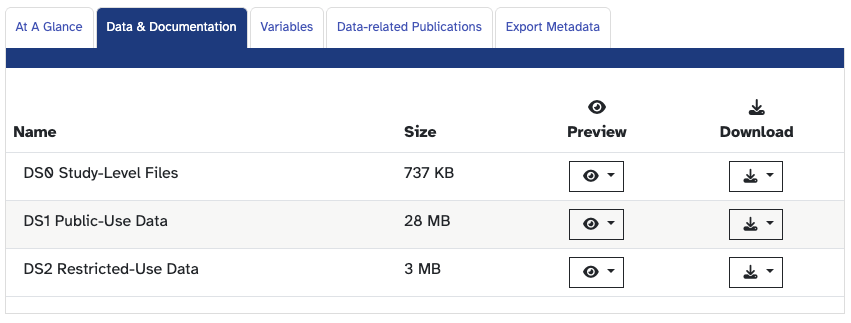
\includegraphics[keepaspectratio]{./images/Lab_01/dnd.png}}
\item
  Download the R version of the Public use data
  \pandocbounded{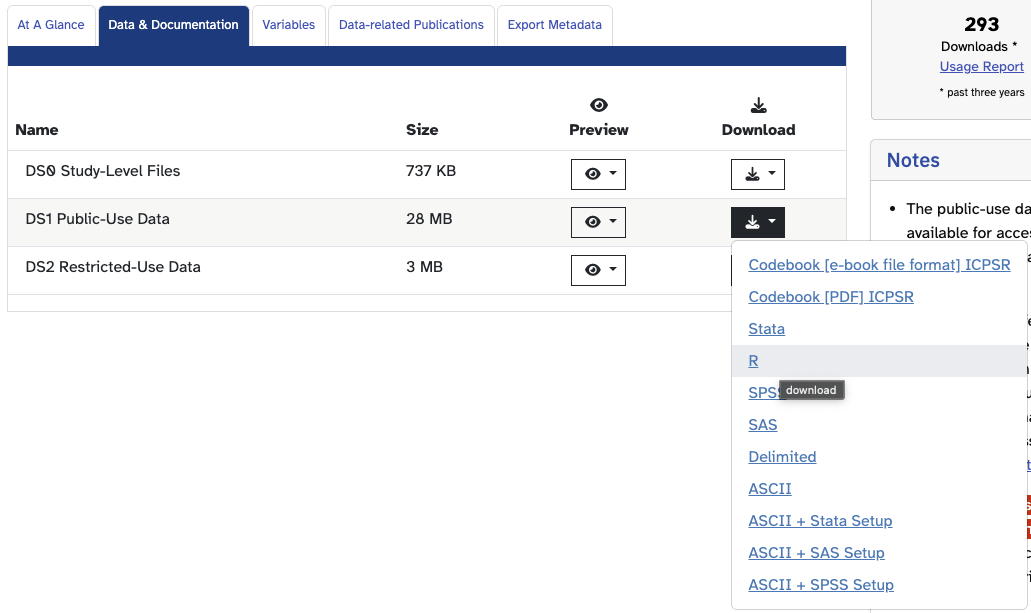
\includegraphics[keepaspectratio]{./images/Lab_01/download.png}}
\item
  Read and agree to the Terms of Use. After this, you will be redirected
  to a new page.
\item
  Log into ICPSR by clicking ``Access through your institution''. You
  should be taken to a new page where you need to select ``Oregon Health
  \& Science University''
  \pandocbounded{
\includegraphics[keepaspectratio]{./images/Lab_01/ICPSR.png}}
\item
  Login using standard OHSU login. Then the download should begin!
\item
  Make sure to move this into your project folder under the Data folder.
\item
  Take a look at the folders/files you just downloaded. Make sure to
  locate and understand the difference between the Codebook,
  Questionnaire, and User Guide. (Note that the website also contains
  the codebook if you go to the variable tab. I think the online one has
  an easier user interface than the pdf.)
\item
  Read the User Guide! There is some important information about the
  data and how to use it.
\end{enumerate}

\begin{tcolorbox}[enhanced jigsaw, toptitle=1mm, toprule=.15mm, leftrule=.75mm, bottomtitle=1mm, breakable, opacityback=0, titlerule=0mm, title=\textcolor{quarto-callout-important-color}{\faExclamation}\hspace{0.5em}{Task}, arc=.35mm, colback=white, rightrule=.15mm, left=2mm, colbacktitle=quarto-callout-important-color!10!white, coltitle=black, opacitybacktitle=0.6, colframe=quarto-callout-important-color-frame, bottomrule=.15mm]

No task to report back on. Just make sure you have the data and read the
User Guide!

\end{tcolorbox}

\subsubsection{Decide on your project
type}\label{decide-on-your-project-type}

In Lab 4, you will need to build a model for your outcome. That's really
far away from this lab, BUT we will have two options for model building
in Lab 4 that affects the work you do in this lab.

For this project, you may either:

\begin{enumerate}
\def\labelenumi{\arabic{enumi}.}
\tightlist
\item
  Use LASSO regression to build a prediction model with no interactions
\item
  Use Purposeful model selection to build an association model with at
  least one interaction
\end{enumerate}

We will discuss prediction modeling in Lesson 14 of this class. We
discussed association modeling in BSTA 512/612, also Lesson 14.

I highly suggest picking the model selection strategy based on
\textbf{your desired learning objectives}:

\begin{enumerate}
\def\labelenumi{\arabic{enumi}.}
\tightlist
\item
  \textbf{LASSO regression} will help stretch your R coding and machine
  learning skills. You will not answer a research question about the
  relationship between a variable and food insecurity. You will ask:
  What variables are most important for predicting food insecurity?
\item
  \textbf{Purposeful model selection} will allow you to cement many
  concepts that we learned within 512/612 and 513/613. You will answer a
  research question about the relationship between a variable and food
  insecurity.
\end{enumerate}

You can change your mind about which model selection strategy you want
to use later on, but your dataset will change a little.

\begin{tcolorbox}[enhanced jigsaw, toptitle=1mm, toprule=.15mm, leftrule=.75mm, bottomtitle=1mm, breakable, opacityback=0, titlerule=0mm, title=\textcolor{quarto-callout-important-color}{\faExclamation}\hspace{0.5em}{Task}, arc=.35mm, colback=white, rightrule=.15mm, left=2mm, colbacktitle=quarto-callout-important-color!10!white, coltitle=black, opacitybacktitle=0.6, colframe=quarto-callout-important-color-frame, bottomrule=.15mm]

Pick between LASSO regression and purposeful model selection. You can
just write your choice.

\end{tcolorbox}

\subsubsection{Decide on list of variables to focus on}\label{sec-pred}

From the codebook, I want you to explore the variables and create a list
of 10 predictors that you would like to focus on. Our outcome is
\texttt{FOOD\_INSEC} so we cannot use this as a predictor. Feel free to
take a look at the
\href{https://www.urban.org/policy-centers/health-policy-center/projects/well-being-and-basic-needs-survey}{Urban
Institute's list of publications} to get ideas of variables and
relationships.

There are a few requirements for your predictors:

\begin{itemize}
\tightlist
\item
  1 variable must be a numeric (i.e.~\texttt{PPAGE})
\item
  1 variable must be binary
\item
  1 variable must be multi-level categorical (categorical with more than
  2 groups)
\item
  You must choose at least 10 predictors (does not include the outcome)
\end{itemize}

There is a
\href{https://www.icpsr.umich.edu/web/HMCA/studies/38759/datasets/0001/variables/ID?archive=HMCA}{good
online version of the codebook} with information about the variables. I
have linked you to the ID varaible, but you can take a look at all the
other variables using the left hand side navigator:

\pandocbounded{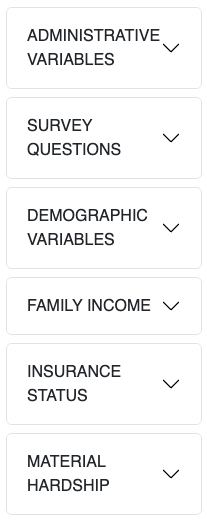
\includegraphics[keepaspectratio]{./images/Lab_01/nav.png}}

You can look under survey questions to get a better sense of how
questions were asked, but please stick to variables under Demographic
Variables, Family Income, Insurance Status, and Material Hardship. Do
not choose variables from the Administrative levels, Survey Questions,
nor School Enrollment or Child Care variables. May leave in the
\texttt{ID} variable for easier tracking on individuals, but it does not
count towards the 10 predictors.

\begin{tcolorbox}[enhanced jigsaw, toptitle=1mm, toprule=.15mm, leftrule=.75mm, bottomtitle=1mm, breakable, opacityback=0, titlerule=0mm, title=\textcolor{quarto-callout-important-color}{\faExclamation}\hspace{0.5em}{Task}, arc=.35mm, colback=white, rightrule=.15mm, left=2mm, colbacktitle=quarto-callout-important-color!10!white, coltitle=black, opacitybacktitle=0.6, colframe=quarto-callout-important-color-frame, bottomrule=.15mm]

List the 10 predictors that you plan to use in your analysis. Note the
type of variable (numeric and continuous, counts, binary, or multi-level
categorical)

\end{tcolorbox}

\subsubsection{Get a sense of how you would like to analyze the
data}\label{get-a-sense-of-how-you-would-like-to-analyze-the-data}

For our project, we will examine the association between the food
insecurity and one other variable (our main explanatory variable). From
the above readings, survey information, and your list of predictors in
Section~\ref{sec-pred}, which association are you most interested in
analyzing?

Please write this in the form of a research question statement. Feel
free to copy this sentence and insert your chosen predictor: We will
investigate the association between food insecurity and \_\_\_\_.

\begin{tcolorbox}[enhanced jigsaw, toptitle=1mm, toprule=.15mm, leftrule=.75mm, bottomtitle=1mm, breakable, opacityback=0, titlerule=0mm, title=\textcolor{quarto-callout-important-color}{\faExclamation}\hspace{0.5em}{Task}, arc=.35mm, colback=white, rightrule=.15mm, left=2mm, colbacktitle=quarto-callout-important-color!10!white, coltitle=black, opacitybacktitle=0.6, colframe=quarto-callout-important-color-frame, bottomrule=.15mm]

Complete the following statement to identify your research question:

We will investigate the association between food insecurity and
\_\_\_\_.

\end{tcolorbox}

\subsubsection{\texorpdfstring{Save data for processing with
\texttt{.Rda}}{Save data for processing with .Rda}}\label{save-data-for-processing-with-.rda}

Within this document, or in a separate document, use R to save a copy of
the dataset so that you can process it without changing the raw data.
Recall the file organization that we discussed to set up proper folders.
Include a screenshot showing the new \texttt{.Rda} file within your Data
folder.

\begin{tcolorbox}[enhanced jigsaw, toptitle=1mm, toprule=.15mm, leftrule=.75mm, bottomtitle=1mm, breakable, opacityback=0, titlerule=0mm, title=\textcolor{quarto-callout-important-color}{\faExclamation}\hspace{0.5em}{Task}, arc=.35mm, colback=white, rightrule=.15mm, left=2mm, colbacktitle=quarto-callout-important-color!10!white, coltitle=black, opacitybacktitle=0.6, colframe=quarto-callout-important-color-frame, bottomrule=.15mm]

Include a screenshot showing the new \texttt{.Rda} file within your Data
folder.

\end{tcolorbox}

\subsubsection{Getting data in working
format}\label{getting-data-in-working-format}

You can start by selecting only the variables you will use in your
analysis. Again, you can keep \texttt{ID} in addition to your outcome
and predictors for easy tracking.

Use the following code (with your dataset's name) to remove the
parentheses with values that are in front of the category names. Make
sure to change \texttt{old\_df} and \texttt{new\_df}.

\begin{Shaded}
\begin{Highlighting}[]
\NormalTok{new\_df }\OtherTok{=} \FunctionTok{data.frame}\NormalTok{(}\FunctionTok{lapply}\NormalTok{(old\_df, }\ControlFlowTok{function}\NormalTok{(x) \{}\FunctionTok{gsub}\NormalTok{(}\StringTok{".*) "}\NormalTok{, }\StringTok{""}\NormalTok{, x)\}))}
\end{Highlighting}
\end{Shaded}

\begin{tcolorbox}[enhanced jigsaw, toptitle=1mm, toprule=.15mm, leftrule=.75mm, bottomtitle=1mm, breakable, opacityback=0, titlerule=0mm, title=\textcolor{quarto-callout-important-color}{\faExclamation}\hspace{0.5em}{Task}, arc=.35mm, colback=white, rightrule=.15mm, left=2mm, colbacktitle=quarto-callout-important-color!10!white, coltitle=black, opacitybacktitle=0.6, colframe=quarto-callout-important-color-frame, bottomrule=.15mm]

\begin{itemize}
\tightlist
\item
  Select the variables that will be used in your analysis and make a new
  dataset. Include the code that you used.
\item
  Remove the parentheses with values that are in front of the category
  names.
\end{itemize}

\end{tcolorbox}

\subsubsection{Explore the outcome and
predictors}\label{explore-the-outcome-and-predictors}

The codebook online gives some nice plots of each variable. Please take
a look at the codebook online to see the spread of each variable. Make
note of any categorical variables that have less than 100 observations
in a group. This may cause issues in our analysis later.

\begin{tcolorbox}[enhanced jigsaw, toptitle=1mm, toprule=.15mm, leftrule=.75mm, bottomtitle=1mm, breakable, opacityback=0, titlerule=0mm, title=\textcolor{quarto-callout-important-color}{\faExclamation}\hspace{0.5em}{Task}, arc=.35mm, colback=white, rightrule=.15mm, left=2mm, colbacktitle=quarto-callout-important-color!10!white, coltitle=black, opacitybacktitle=0.6, colframe=quarto-callout-important-color-frame, bottomrule=.15mm]

\begin{itemize}
\tightlist
\item
  To check that you have looked that the variables, please report the
  percent of respondents that were food insecure in the past 12 months.
\item
  List any categorical variables that have less than 100 observations in
  a group
\end{itemize}

\end{tcolorbox}

\subsubsection{Compile above work into an
introduction}\label{compile-above-work-into-an-introduction}

Please
\href{https://www.scribbr.com/research-paper/research-paper-introduction/}{check
out this source} for what a research article introduction includes and
how to organize it. The only thing I would add is mentioning the
Well-Being and Basic Needs Survey.

\begin{tcolorbox}[enhanced jigsaw, toptitle=1mm, toprule=.15mm, leftrule=.75mm, bottomtitle=1mm, breakable, opacityback=0, titlerule=0mm, title=\textcolor{quarto-callout-important-color}{\faExclamation}\hspace{0.5em}{Task}, arc=.35mm, colback=white, rightrule=.15mm, left=2mm, colbacktitle=quarto-callout-important-color!10!white, coltitle=black, opacitybacktitle=0.6, colframe=quarto-callout-important-color-frame, bottomrule=.15mm]

Write an introduction to the analysis using 3-5 bullets.

\end{tcolorbox}




\end{document}
